\documentclass[a4paper]{article}

\usepackage[T1]{fontenc}
\usepackage[italian]{babel}
\usepackage[latin1]{inputenc}
\usepackage{graphicx}
\usepackage{float}
\usepackage[margin=2 cm]{geometry}
\usepackage{multirow}
\usepackage{multicol}
\usepackage{textcomp}
\usepackage{caption}
\usepackage{amsmath}
\usepackage{mathtools}
\author{Alberto Bordin, Giulio Cappelli}
\title{Olografia}
\date{13-17 Novembre 2017}
\newcommand{\minitab}[2][l]{\begin{tabular}#1 #2\end{tabular}}


\begin{document}
	\maketitle
	
	\begin{abstract}
		 
	\end{abstract}

\begin{multicols}{2}	
\section{Teoria}
L'olografia � basata sulla registrazione di fase e ampiezza di un'onda elettromagnetica $a(x,y)= |a(x, y)|e^{i\phi(x,y)}$ su di un supporto che giace nel piano x-y, in modo da poter poi ricostruire l'immagine. Il supporto in questione � una lastra fotografica sensibile all'intensit� incidente, quindi � necessaria un'onda di riferimento $A(x,y)= |A(x, y)|e^{i\psi(x,y)}$. Infatti l'interferenza tra il fascio di riferimento e il fascio diffuso dall'oggetto provoca un pattern d'interferenza che contiene tutta l'informazione su ampiezza e fase in quanto l'intensit� incidente sulla lastra risulta essere:
\begin{equation}
\begin{aligned}
I(x,y)=|A(x,y)+a(x,y)|^2=\\= |A(x, y)|^2+|a(x, y)|^2+|a|^2+aA^*+Aa^*
\end{aligned}
\end{equation}
Assumendo che la trasmettivit� della lastra sia lineare con l'intensit� incidente, $t=\gamma I$, si ha:
\begin{equation}
t(x,y)=t_{ref}+\gamma(|a|^2+aA^*+Aa^*)
\end{equation}
dove $t_{ref} = \gamma|A|^2$ � la trasmettivit� di background dovuta all'onda di riferimento. 

\'E quindi possibile ricostruire l'immagine registrata utilizzando in trasmissione un'onda di ricostruzione $B(x,y)$, infatti il campo trasmesso �:
\begin{equation}
\begin{aligned}
E_{trasm}=Bt=Bt_{ref}+\gamma(B|a|^2+BaA^*+BAa^*)=\\=U_1+U_2+U_3+U_4
\end{aligned}
\end{equation}

Utilizzando come fascio di ricostruzione lo stesso fascio di luce usato per il riferimento e assumendo che $|A|^2$ sia costante su tutta la lastra, si hanno due termini lineari rispettivamente in $a$ e $a^*$ che contengono tutta l'informazione sull'oggetto in esame:
\begin{equation}
U_3=\gamma|A|^2a \qquad U_4=\gamma A^2a^*
\end{equation}
Se vogliamo quindi ricostruire e osservare l'immagine occorre separare spazialmente queste due componenti del campo trasmesso e per farlo si utilizza lo schema mostrato in Figura \ref{fig:schema} che riprende quello dell'ologramma di Leith-Uptanieks.

\end{multicols}

\begin{figure}[H]
\centering
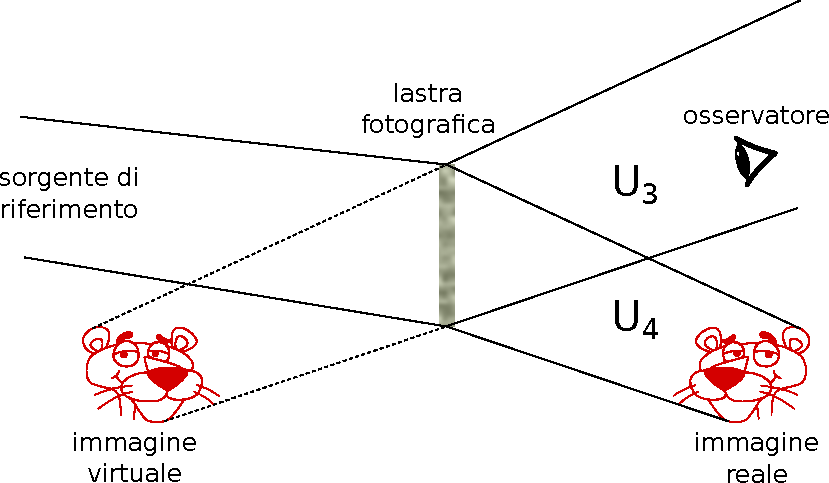
\includegraphics[width=0.9\textwidth]{olografia_virtuale_reale.pdf}
\caption{Schema olografia di Leith-Uptanieks}
\label{fig:schema}
\end{figure}
 
 \newpage
\section{Apparato sperimentale}

\begin{figure}[H]
\centering
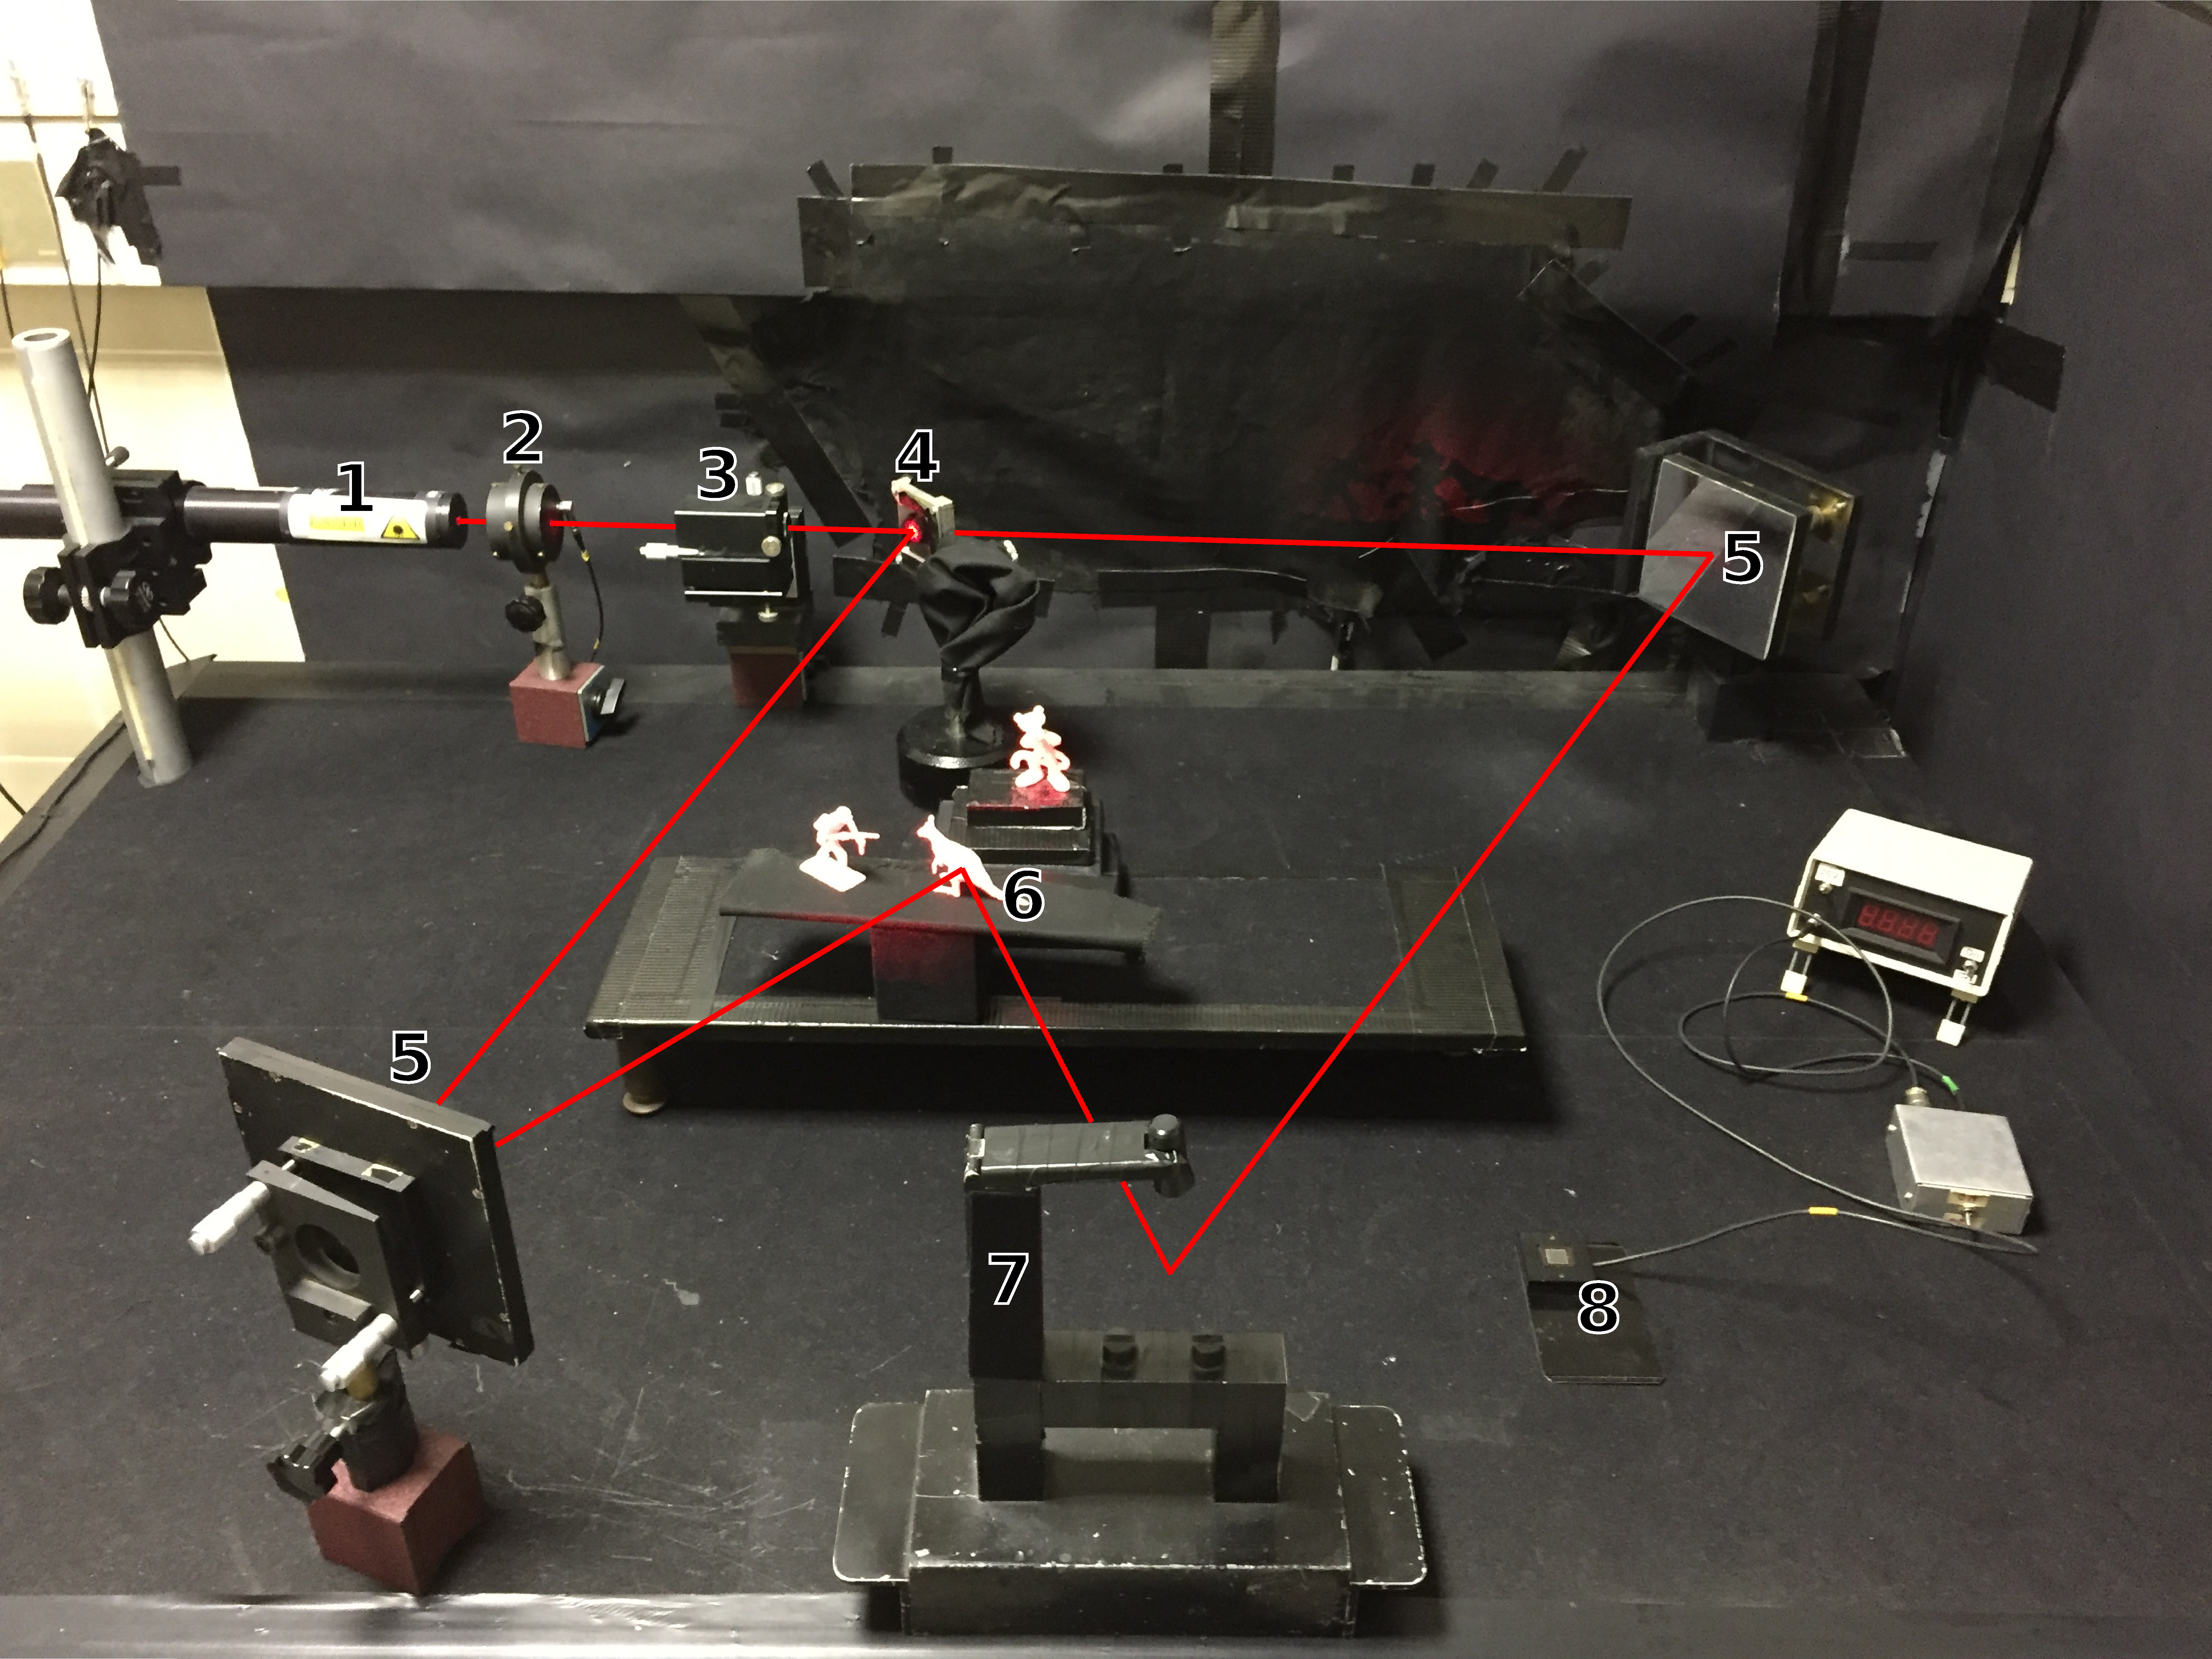
\includegraphics[width=0.9\textwidth]{apparato_olografia.pdf}
\caption{Schema olografia di Leith-Uptanieks. In rosso � tracciato il percorso del fascio laser.}
\label{fig:apparato}
\end{figure}

\begin{multicols}{2}

L'apparato a disposizione � riportato in Figura \ref{fig:apparato} ed � composto da:

\begin{enumerate}
\item Laser He-Ne ($\lambda$=633 nm) di potenza $\sim$15 mW e con una lunghezza di coerenza di $\sim$1 m.
\item Shutter, azionabile dall'esterno, per oscurare completamente il fascio.
\item Obbiettivo x20 e filtro spaziale (\emph{pin-hole}). Il primo trasforma quella che, date le distanze in gioco, pu� essere considerata un'onda piana in un'onda sferica per ottenere interferenza al finito. Il secondo � posizionato nel fuoco della lente divergente ed ha un diametro 12.5 $\mu$m per selezionare il modo TEM$_{00}$, grazie al quale si ha un'illuminazione uniforme. 
\item Beam splitter che trasmette il 5\% del fascio come riferimento e ne riflette il 95\%, che viene poi indirizzato sull'oggetto.
\item Specchi per indirizzare i due fasci uno sulla lastra e uno sull'oggetto.
\item Oggetto di cui vogliamo fare l'olografia; dipinto di bianco cos� da massimizzare la riflessione della luce su di esso.
\item Supporto per la lastra fotografica.
\item Rivelatore al silicio con una superficie attiva di 1 cm$^2$ montato su un supporto che permette di misurare l'intensit� incidente su tutta la superficie della lastra. 
\begin{figure}[H]
\centering
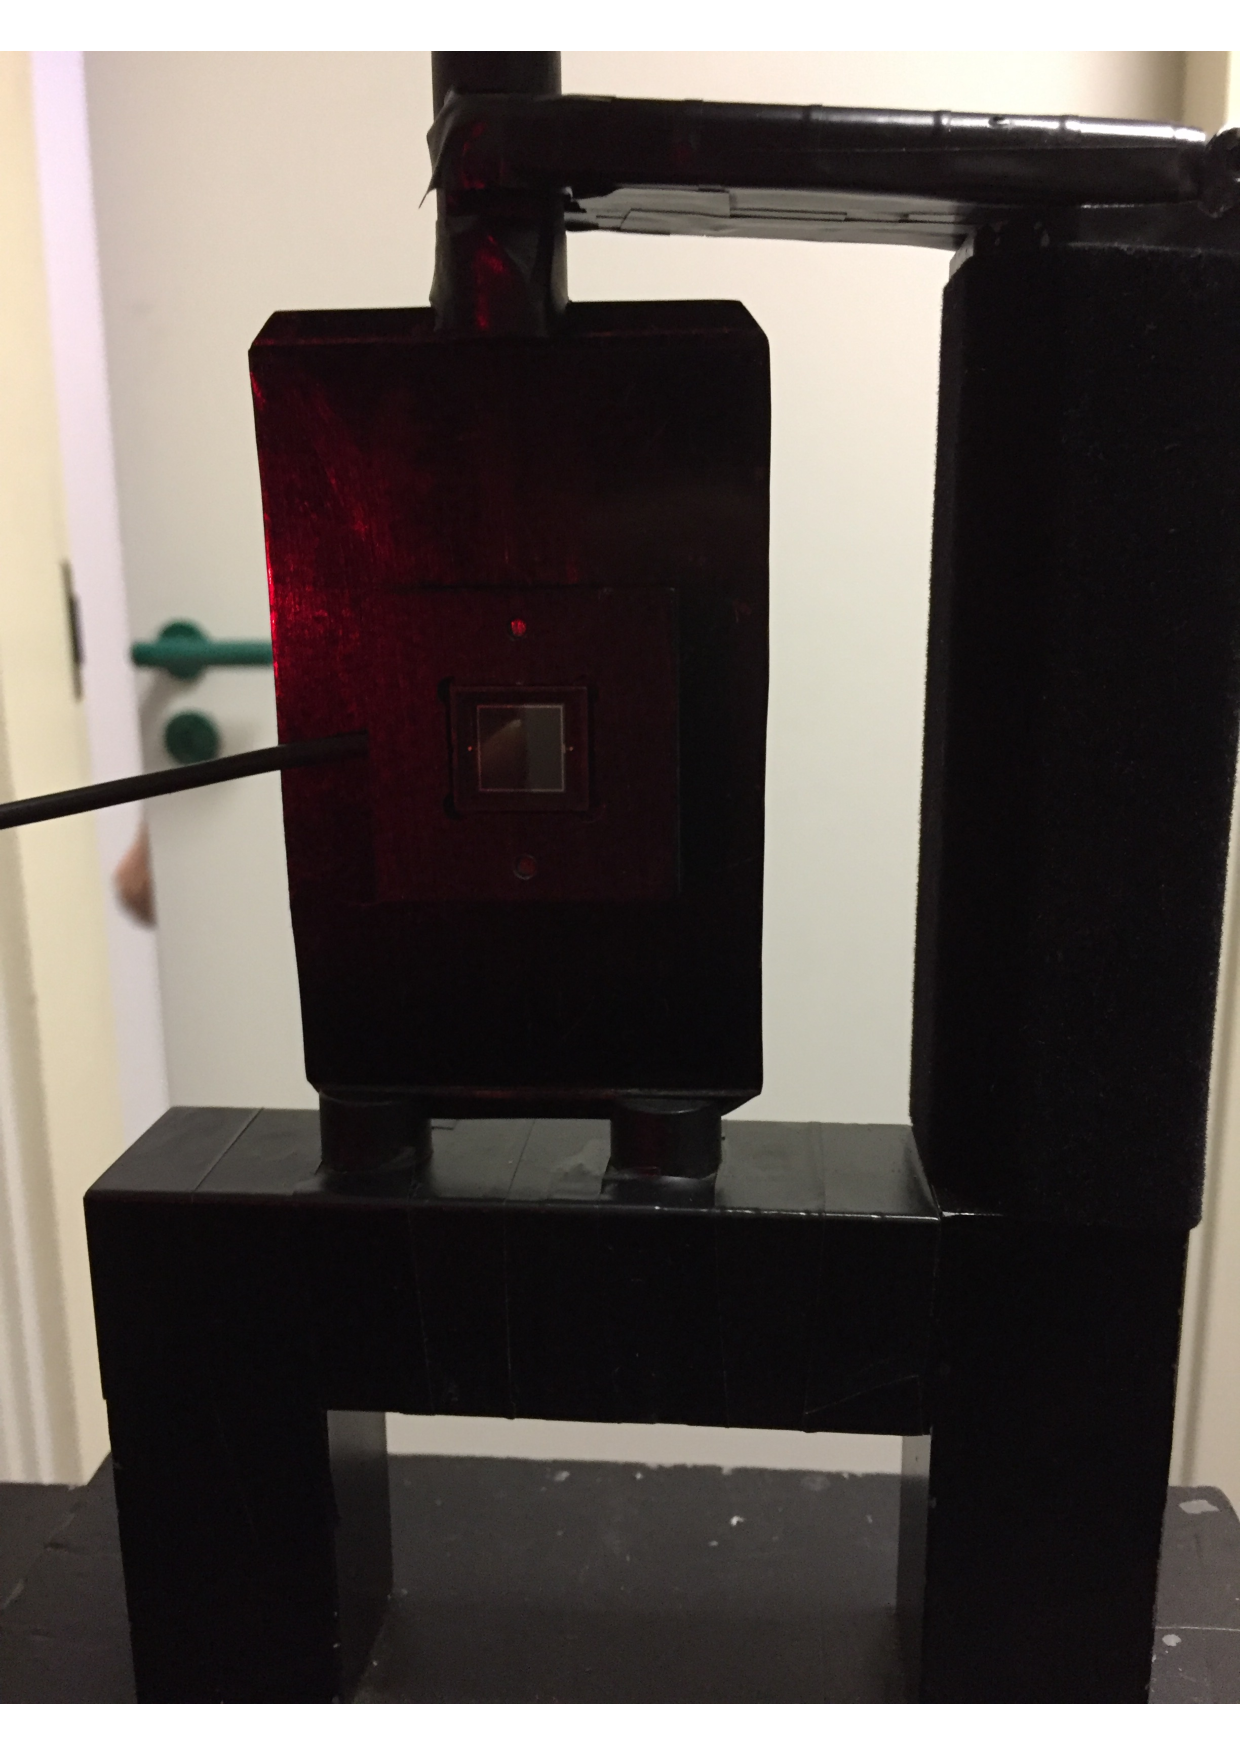
\includegraphics[width=0.4\textwidth]{rivelatore.pdf}
\end{figure}
Il fotodiodo restituisce una tensione che � possibile convertire in una potenza per cm$^2$ grazie alla curva di taratura presente in laboratorio:
\begin{equation}
P[\mu W] =  -0.16925 + 2.6592V_{mis}
\label{eq:taratura}
\end{equation}
\begin{figure}[H]
\centering
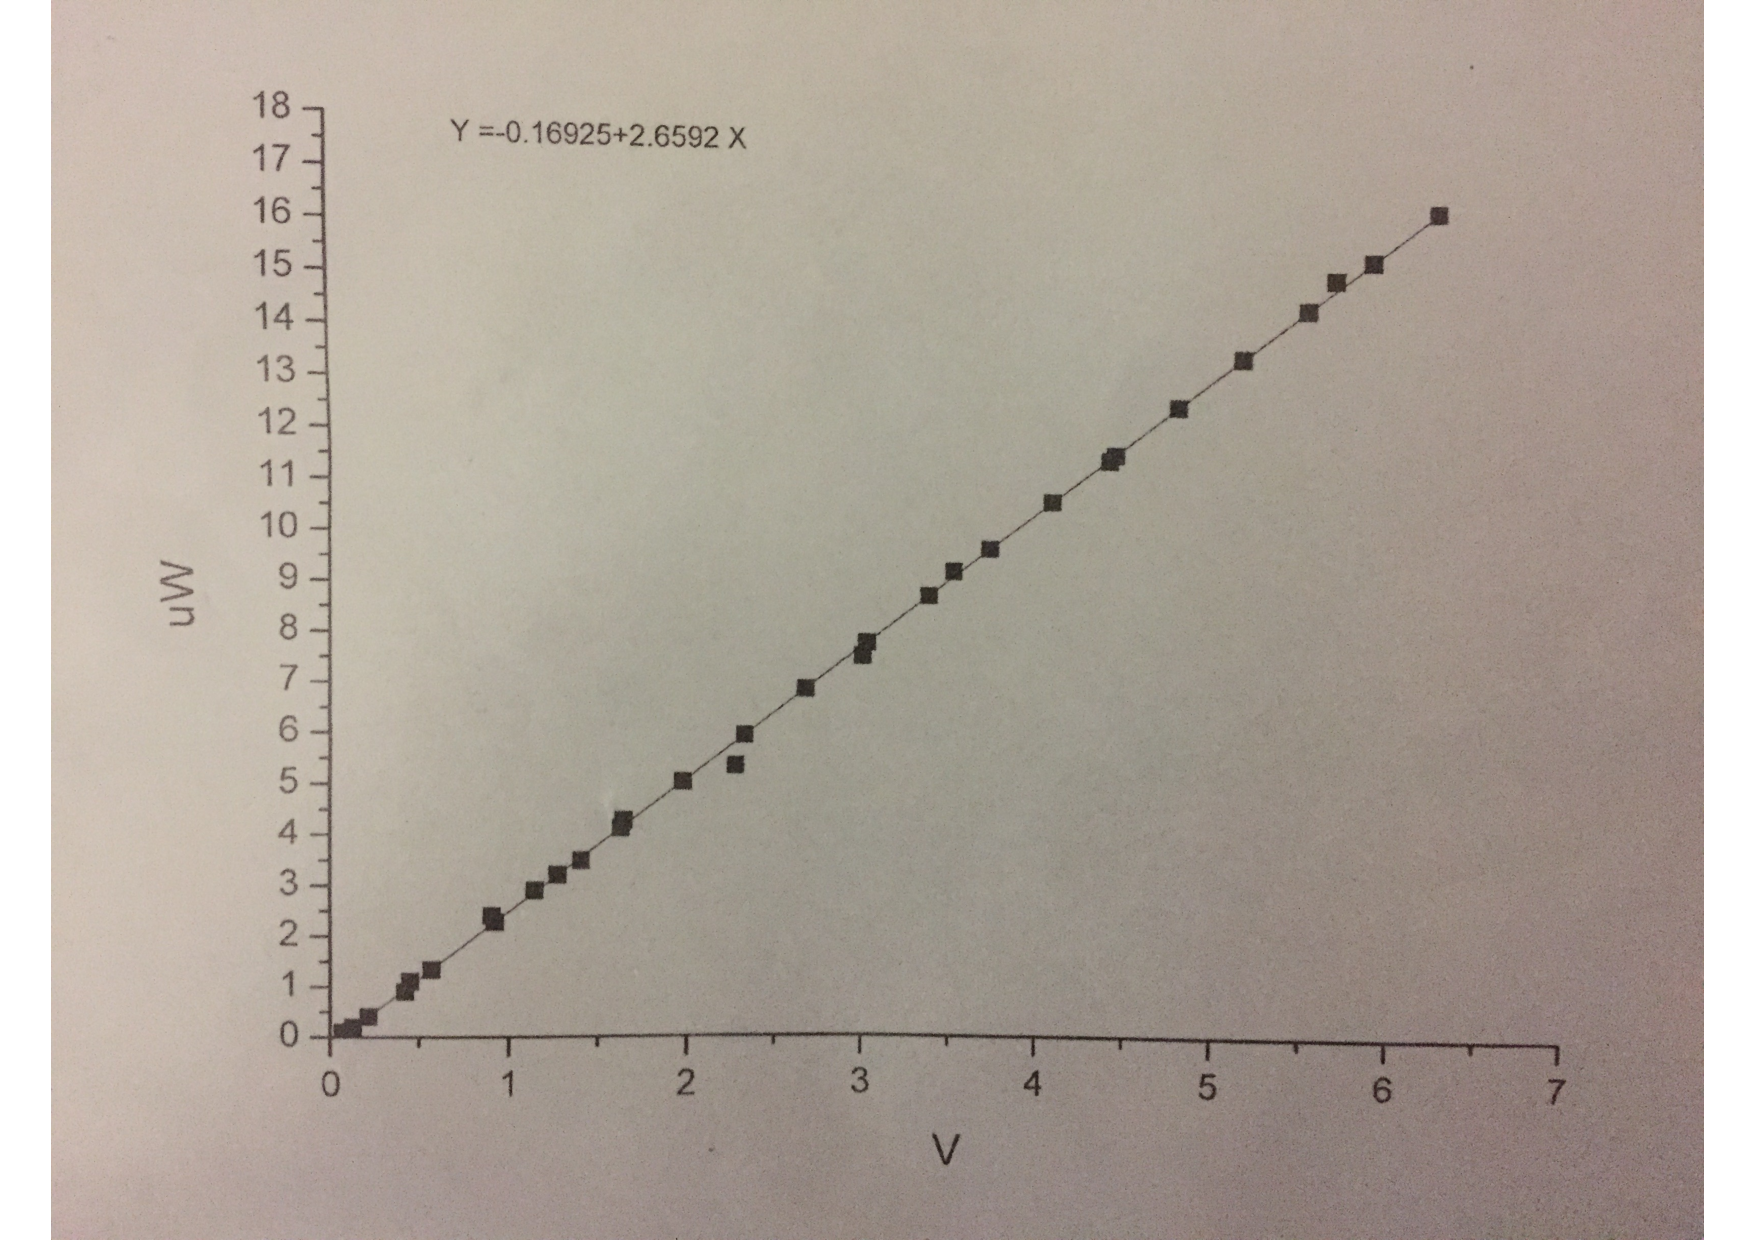
\includegraphics[width=0.4\textwidth]{taratura.pdf}
\end{figure}
\end{enumerate}

Abbiamo inoltre a disposizione 4 lastre fotografiche ai sali d'argento; non esistono infatti dispositivi di acquisizione elettronici con la risoluzione necessaria a registrare l'interferenza di luce visibile.

\section{Accorgimenti sperimentali}

Come scritto, utilizziamo lo stesso fascio laser diviso in ampiezza come onda di riferimento e onda incidente sull'oggetto. \'E quindi necessario porre particolare attenzione al cammino ottico percorso dai due fasci; infatti la fase relativa fra il fascio proveniente dall'oggetto e quello di riferimento deve essere ben definita. Per questo la differenza di cammino tra i due fasci deve essere molto minore della lunghezza di coerenza del laser He-Ne. Si deve cio� avere:
\begin{equation}
A+B = C+D+E
\label{eq:distanza}
\end{equation}

\'E inoltre necessario calcolare il corretto tempo di esposizione della lastra. Per farlo serve conoscere la densit� superficiale di energia necessaria per un annerimento ottimale che il professore ci ha detto essere 50 $\frac{\mu J}{cm^2}$.

Conoscendo la potenza incidente sulla lastra � quindi possibile ricavare il tempo di esposizione:
\begin{equation}
t [s] = \frac{50 [\mu J]}{P[\mu W]} = \frac{50 [\mu J]}{-0.16925 + 2.6592V_{mis}}
\label{eq:tempo}
\end{equation}

Come spiegato nella parte di teoria la lastra deve essere illuminata in modo uniforme, per questo sono state misurate le intensit� $I_r$, $I_o$ e $I_{tot}$, rispettivamente, del fascio di riferimento, della luce diffusa dall'oggetto e quella totale. 
Misurando separatamente $I_r$ e $I_o$ ci si � preoccupati anche di avere un buon rapporto segnale rumore verificando che l'intensit� del fascio di riferimento fosse maggiore di quella del fascio oggetto.

\subsection{Elaborazione lastra}

La lastra fotografica non deve essere esposta alla luce ambientale prima di essere impressionata e sviluppata.
Una volta impressionata, la lastra deve essere inserita in un contenitore in modo tale che non venga esposta alla luce e che possa essere quindi sviluppata senza essere danneggiata. 

Il processo di sviluppo � costituito da 4 fasi che prevedono di riempire il contenitore con 3 diversi liquidi:
\begin{itemize}
\item Riempire il contenitore con il liquido di sviluppo e attendere 5 minuti
\item Riempire il contenitore con acqua distillata e attendere 5 minuti
\item Riempire il contenitore con il liquido di fissaggio e attendere 5 minuti
\item Riempire il contenitore con acqua distillata e attendere 5 minuti
\end{itemize}

Dopo questi 4 passaggi � possibile estrarre la lastra dal contenitore e una volta asciutta pu� essere osservata posizionandola nuovamente sul supporto e illuminandola col fascio di ricostruzione.

\section{Misure preliminari}
Prima di posizionare ed impressionare la lastra fotografica sono necessarie alcune misure preliminari come evidenziato negli accorgimenti sperimentali.

Per ognuna delle 4 lastre impressionate sono state eseguite le seguenti misure:

\begin{itemize}
\item Abbiamo misurate le distanze A, B, C, D, E in modo che fosse verificata la relazione \ref{eq:distanza}
\item Abbiamo interrotto il fascio che incideva sull'oggetto e misurato l'intensit� $I_r$ del fascio di riferimento.
\item Abbiamo interrotto il fascio di riferimento e misurato l'intensit� $I_o$ della luce diffusa dall'oggetto.
\item Abbiamo misurato l'intensit� totale $I_{tot}$ incidente sulla lastra.
\item Abbiamo calcolato la potenza totale $P_{tot}$ incidente sulla lastra utilizzando l'equazione \ref{eq:taratura}
\item Abbiamo calcolato il tempo di esposizione considerando il valore centrale di $P_{tot}$ utilizzando l'equazione \ref{eq:tempo}
\end{itemize}

Nelle seguenti sezioni sono riportate varie tabelle in cui sono presenti tutti i valori misurati per ognuna delle quattro lastre.

\newpage
\section{Olografia statica}

Abbiamo utilizzato le prime due lastre per effettuare l'olografia di alcuni oggetti immobili e posizionati come in Figura \ref{fig:apparato}.

\subsection{Soldatino con lancia}

Come primo oggetto abbiamo scelto un soldatino dotato di una lancia.

\begin{table}[H]
\centering
\begin{tabular}{ccccc}
	\hline
	A & B & C & D & E \\
	\hline
	\hline
	  60.0 & 92.5 & 78.5 & 38.0 & 36.0  \\
	\hline
\end{tabular}
\caption*{Distanze in cm con un errore di 0.5 cm}
\end{table}

\begin{table}[H]
\centering
\begin{tabular}{|c|c|c|}
	\hline
	  1.14 &  & 1.12  \\
	\hline
	   & 1.48 &   \\
	\hline
	  1.12 &   & 1.13 \\
	\hline
\end{tabular}
\caption*{Valori di $I_{r}$ espressi in V con un errore di 0.01 V}
\end{table}

\begin{table}[H]
\centering
\begin{tabular}{|c|c|c|}
	\hline
	  56 &   & 59 \\
	\hline
	   & 59 &   \\
	\hline
	  54 &   & 59 \\
	\hline
\end{tabular}
\caption*{Valori di $I_{o}$ espressi in mV con un errore di 1 mV}
\end{table}

\begin{table}[H]
\centering
\begin{tabular}{|c|c|c|}
	\hline
	  1.09 & 1.13  & 1.11  \\
	\hline
	 1.43  & 1.50 &  1.45 \\
	\hline
	  1.21 & 1.26 & 1.24 \\
	\hline
\end{tabular}
\caption*{Valori di $I_{tot}$ espressi in V con un errore di 0.01 V}
\end{table}

\begin{table}[H]
\centering
\begin{tabular}{|c|c|c|}
	\hline
	  2.73 & 2.84 & 2.78  \\
	\hline
	  3.63 & 3.81 & 3.69 \\
	\hline
	  3.04 & 3.18 & 3.13 \\
	\hline
\end{tabular}
\caption*{Valori di $P_{tot}$ espressi in $\mu$W}
\end{table}

Abbiamo cos� ottenuto un tempo di esposizione\\ t = 13 s che ha portato all'ologramma mostrato in Figura \ref{fig:soldatino}:

 \end{multicols}

\begin{figure}[H]
\centering
\includegraphics[width=\textwidth]{soldatino}
\caption{}
\label{fig:soldatino}
\end{figure}

\newpage
\begin{multicols}{2}

\subsection{La caccia}

Per la seconda lastra abbiamo scelto tre oggetti diversi: un canguro, un soldato con un fucile e la pantera rosa. 

\begin{table}[H]
\centering
\begin{tabular}{cccccc}
	\hline
	 Oggetto & A & B & C & D & E \\
	\hline
	\hline
	Soldato & 62.5& 89.5& 77.5&34.5 & 39.0\\
	\hline
	Canguro & - &- &- & 38.5&35.5 \\
	\hline
	Pantera & -& -& -&50.0 & 46.0\\
\end{tabular}
\caption*{Distanze in cm con un errore di 0.5 cm}
\end{table}

\begin{table}[H]
\centering
\begin{tabular}{|c|c|c|}
	\hline
	  1.19 & 1.24  &  1.19 \\
	\hline
	  1.50 & 1.54  & 1.49  \\
	\hline
	  1.20 & 1.22 & 1.19  \\
	\hline
\end{tabular}
\caption*{Valori di $I_{r}$ espressi in V con un errore di 0.01 V}
\end{table}

\begin{table}[H]
\centering
\begin{tabular}{|c|c|c|}
	\hline
	  67 & 69  & 70  \\
	\hline
	  68 & 70 &  71 \\
	\hline
	  69 & 68 & 71 \\
	\hline
\end{tabular}
\caption*{Valori di $I_{o}$ espressi in mV con un errore di 1 mV}
\end{table}

\begin{table}[H]
\centering
\begin{tabular}{|c|c|c|}
	\hline
	  1.25 & 1.30  & 1.25 \\
	\hline
	  1.56 & 1.59 & 1.52 \\
	\hline
	 1.25  & 1.27 & 1.24 \\
	\hline
\end{tabular}
\caption*{Valori di $I_{tot}$ espressi in V con un errore di 0.01 V}
\end{table}

\begin{table}[H]
\centering
\begin{tabular}{|c|c|c|}
	\hline
	 3.15  & 3.28  & 3.15 \\
	\hline
	   3.98 & 4.06  & 3.87  \\
	\hline
	 3.15  & 3.21  &  3.13 \\
	\hline
\end{tabular}
\caption*{Valori di $P_{tot}$ espressi in $\mu$W}
\end{table}

Abbiamo cos� ottenuto un tempo di esposizione \\t = 12 s che ha portato all'ologramma mostrato in Figura \ref{fig:caccia}:

 \end{multicols}

\begin{figure}[H]
\centering
\includegraphics[width=\textwidth]{caccia}
\caption{}
\label{fig:caccia}
\end{figure}

\newpage
\begin{multicols}{2}

\section{Olografia dinamica}
Le restanti due lastra le abbiamo utilizzate per effettuare due ologrammi dinamici, cio� i due oggetti scelti sono stati posti in due stati diversi per met� tempo di esposizione ciascuno. 

\subsection{Cubo con martelletto}
Il primo oggetto scelto � un cubo dotato di un martelletto che pu� sbatterci sopra. Per effettuare l'ologramma abbiamo preparato la lastra, premuto il martelletto, acceso il laser, lasciato il martelletto e infine spento il laser.

\begin{table}[H]
\centering
\begin{tabular}{ccccc}
	\hline
	A & B & C & D & E \\
	\hline
	\hline
	  62.5 & 89.5 & 78.0 & 39.0 & 35.0  \\
	\hline
\end{tabular}
\caption*{Distanze in cm con un errore di 0.5 cm}
\end{table}

\begin{table}[H]
\centering
\begin{tabular}{|c|c|c|}
	\hline
	 1.24  & 1.29 & 1.25 \\
	\hline
	  1.53 & 1.55 & 1.51 \\
	\hline
	  1.19 & 1.24 & 1.15 \\
	\hline
\end{tabular}
\caption*{Valori di $I_{r}$ espressi in V con un errore di 0.01 V}
\end{table}

\begin{table}[H]
\centering
\begin{tabular}{|c|c|c|}
	\hline
	 51  & 51 & 51 \\
	\hline
	  53 & 52 & 53 \\
	\hline
	  50 & 50 & 50 \\
	\hline
\end{tabular}
\caption*{Valori di $I_{o}$ espressi in mV con un errore di 1 mV}
\end{table}

\begin{table}[H]
\centering
\begin{tabular}{|c|c|c|}
	\hline
	  1.23 & 1.30  & 1.25 \\
	\hline
	  1.55 & 1.58 & 1.54 \\
	\hline
	  1.25 & 1.30 & 1.22 \\
	\hline
\end{tabular}
\caption*{Valori di $I_{tot}$ espressi in V con un errore di 0.01 V}
\end{table}

\begin{table}[H]
\centering
\begin{tabular}{|c|c|c|}
	\hline
	 3.10  & 3.29  &  3.15 \\
	\hline
	  3.95 &  4.03 &  3.93 \\
	\hline
	  3.15 & 3.29  &  3.07 \\
	\hline
\end{tabular}
\caption*{Valori di $P_{tot}$ espressi in $\mu$W}
\end{table}

Abbiamo cos� ottenuto un tempo di esposizione \\t = 12 s diviso in due parti da 6 s ciascuna che ha portato all'ologramma mostrato in Figura \ref{fig:martelletto}:

 \end{multicols}

\begin{figure}[H]
\centering
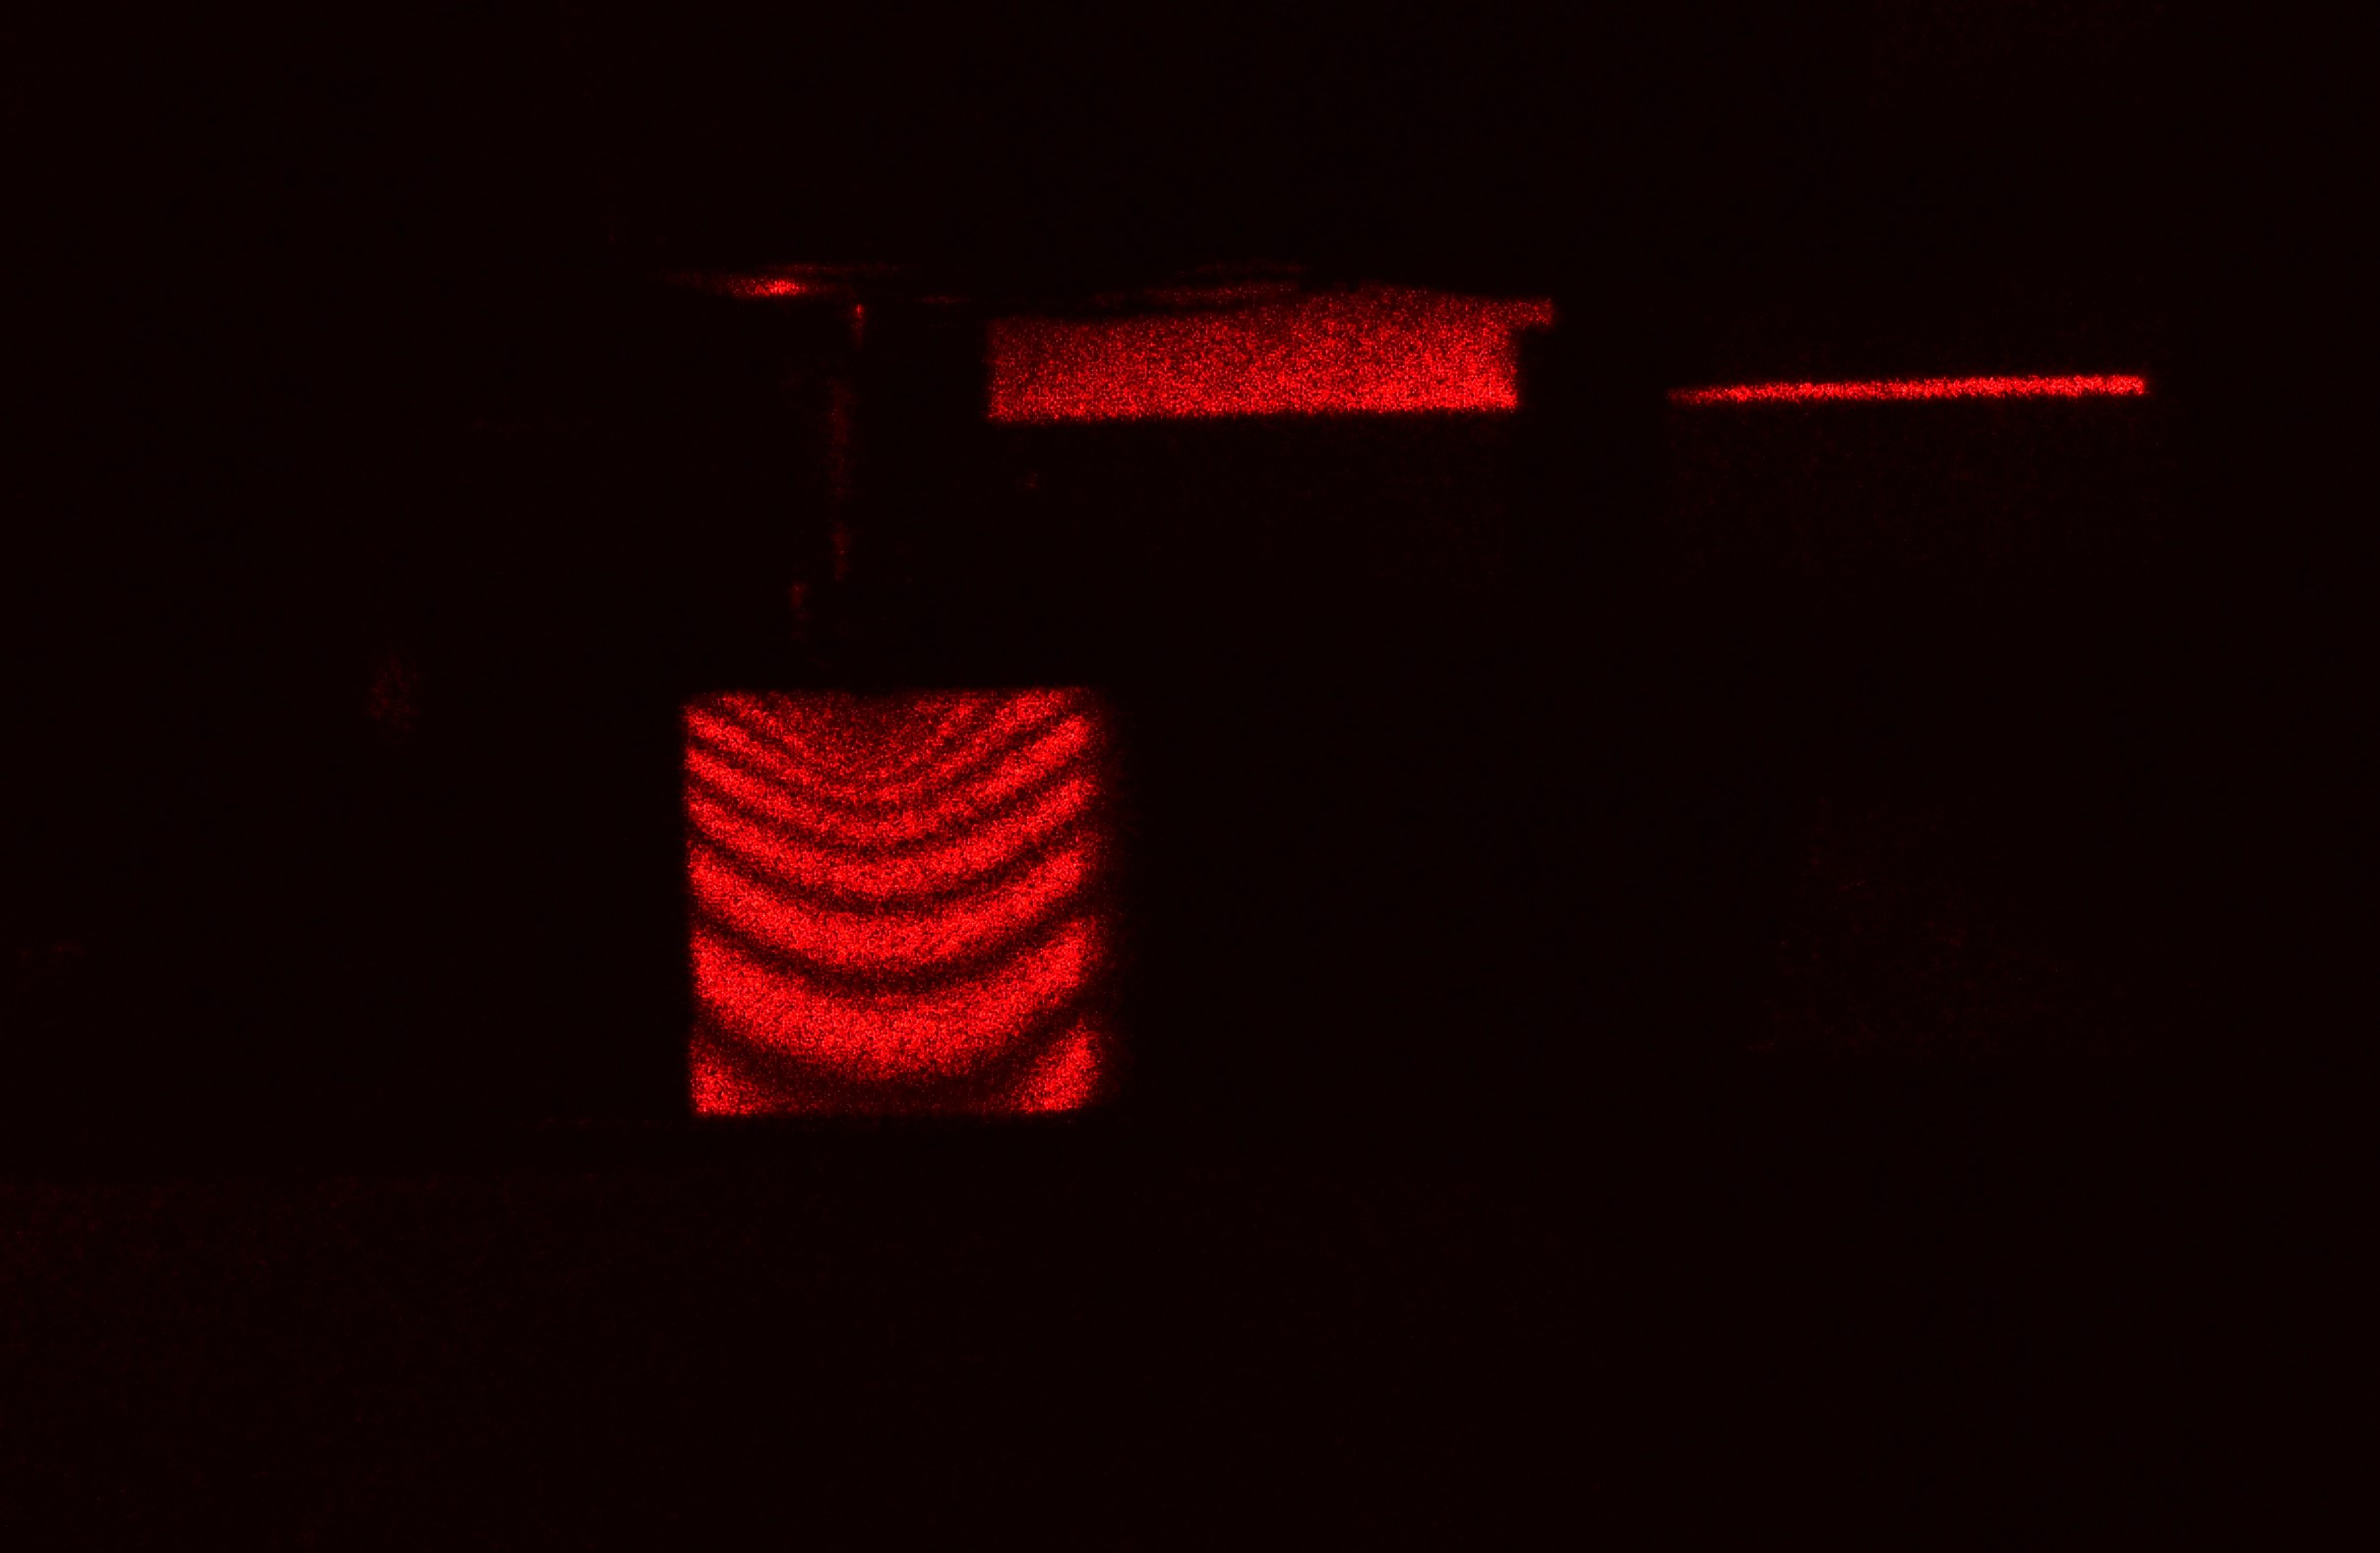
\includegraphics[width=\textwidth]{cubo}
\caption{}
\label{fig:martelletto}
\end{figure}

\newpage
\begin{multicols}{2}

\subsection{Altoparlante}

Abbiamo utilizzato l'ultima lastra a nostra disposizione per effettuare l'olografia di un altoparlante collegato ad un generatore di funzioni impostato a 783 Hz ( un Sol5). Come per il cubo abbiamo tenuto acceso l'altoparlante per la prima met� del tempo di esposizione e lo abbiamo tenuto spento durante la seconda met�. 

\begin{table}[H]
\centering
\begin{tabular}{ccccc}
	\hline
	A & B & C & D & E \\
	\hline
	\hline
	  63.0 & 87.5 & 69.0 & 36.5 & 44.0  \\
	\hline
\end{tabular}
\caption*{Distanze in cm con un errore di 0.5 cm}
\end{table}


\begin{table}[H]
\centering
\begin{tabular}{|c|c|c|}
	\hline
	  1.24 & 1.31 & 1.28 \\
	\hline
	 1.58 & 1.61 & 1.57 \\
	\hline
	  1.26 & 1.33 & 1.25 \\
	\hline
\end{tabular}
\caption*{Valori di $I_{r}$ espressi in V con un errore di 0.01 V}
\end{table}

\begin{table}[H]
\centering
\begin{tabular}{|c|c|c|}
	\hline
	  98 & 95 & 96 \\
	\hline
	  94 & 97 & 100 \\
	\hline
	  93 & 97 & 99 \\
	\hline
\end{tabular}
\caption*{Valori di $I_{o}$ espressi in mV con un errore di 1 mV}
\end{table}

\begin{table}[H]
\centering
\begin{tabular}{|c|c|c|}
	\hline
	  1.34 & 1.38 & 1.36 \\
	\hline
	  1.62 & 1.67 & 1.65 \\
	\hline
	  1.29 & 1.38 & 1.30 \\
	\hline
\end{tabular}
\caption*{Valori di $I_{tot}$ espressi in V con un errore di 0.01 V}
\end{table}

\begin{table}[H]
\centering
\begin{tabular}{|c|c|c|}
	\hline
	  3.39 & 3.50  &  3.44 \\
	\hline
	  4.14 &  4.27 &  4.22 \\
	\hline
	  3.26 &  3.50 & 3.29  \\
	\hline
\end{tabular}
\caption*{Valori di $P_{tot}$ espressi in $\mu$W}
\end{table}
Abbiamo cos� ottenuto un tempo di esposizione \\t = 11.7 s che ha portato all'ologramma mostrato in Figura \ref{fig:altoparlante}:

 \end{multicols}

\begin{figure}[H]
\centering
\includegraphics[width=\textwidth]{altoparlante}
\caption{}
\label{fig:altoparlante}
\end{figure}

\newpage
\begin{multicols}{2}

\section{Lampada spettrale}

Una lampada spettrale � in grado di emettere luce a diverse lunghezze d'onda nel visibile. Osservando l'ologramma in trasmissione, l'interferenza fra la luce di ogni $\lambda$ e il pattern d'interferenza impressionati sulla lastra genera un'immagini spostata rispetto a quella ottenuta col fascio con cui � stata impressionata la lastra. Le immagini relative alle diverse d'onda vengono quindi separate come mostrato in Figura \ref{fig:spettro}:

\end{multicols}

\begin{figure}[H]
\centering
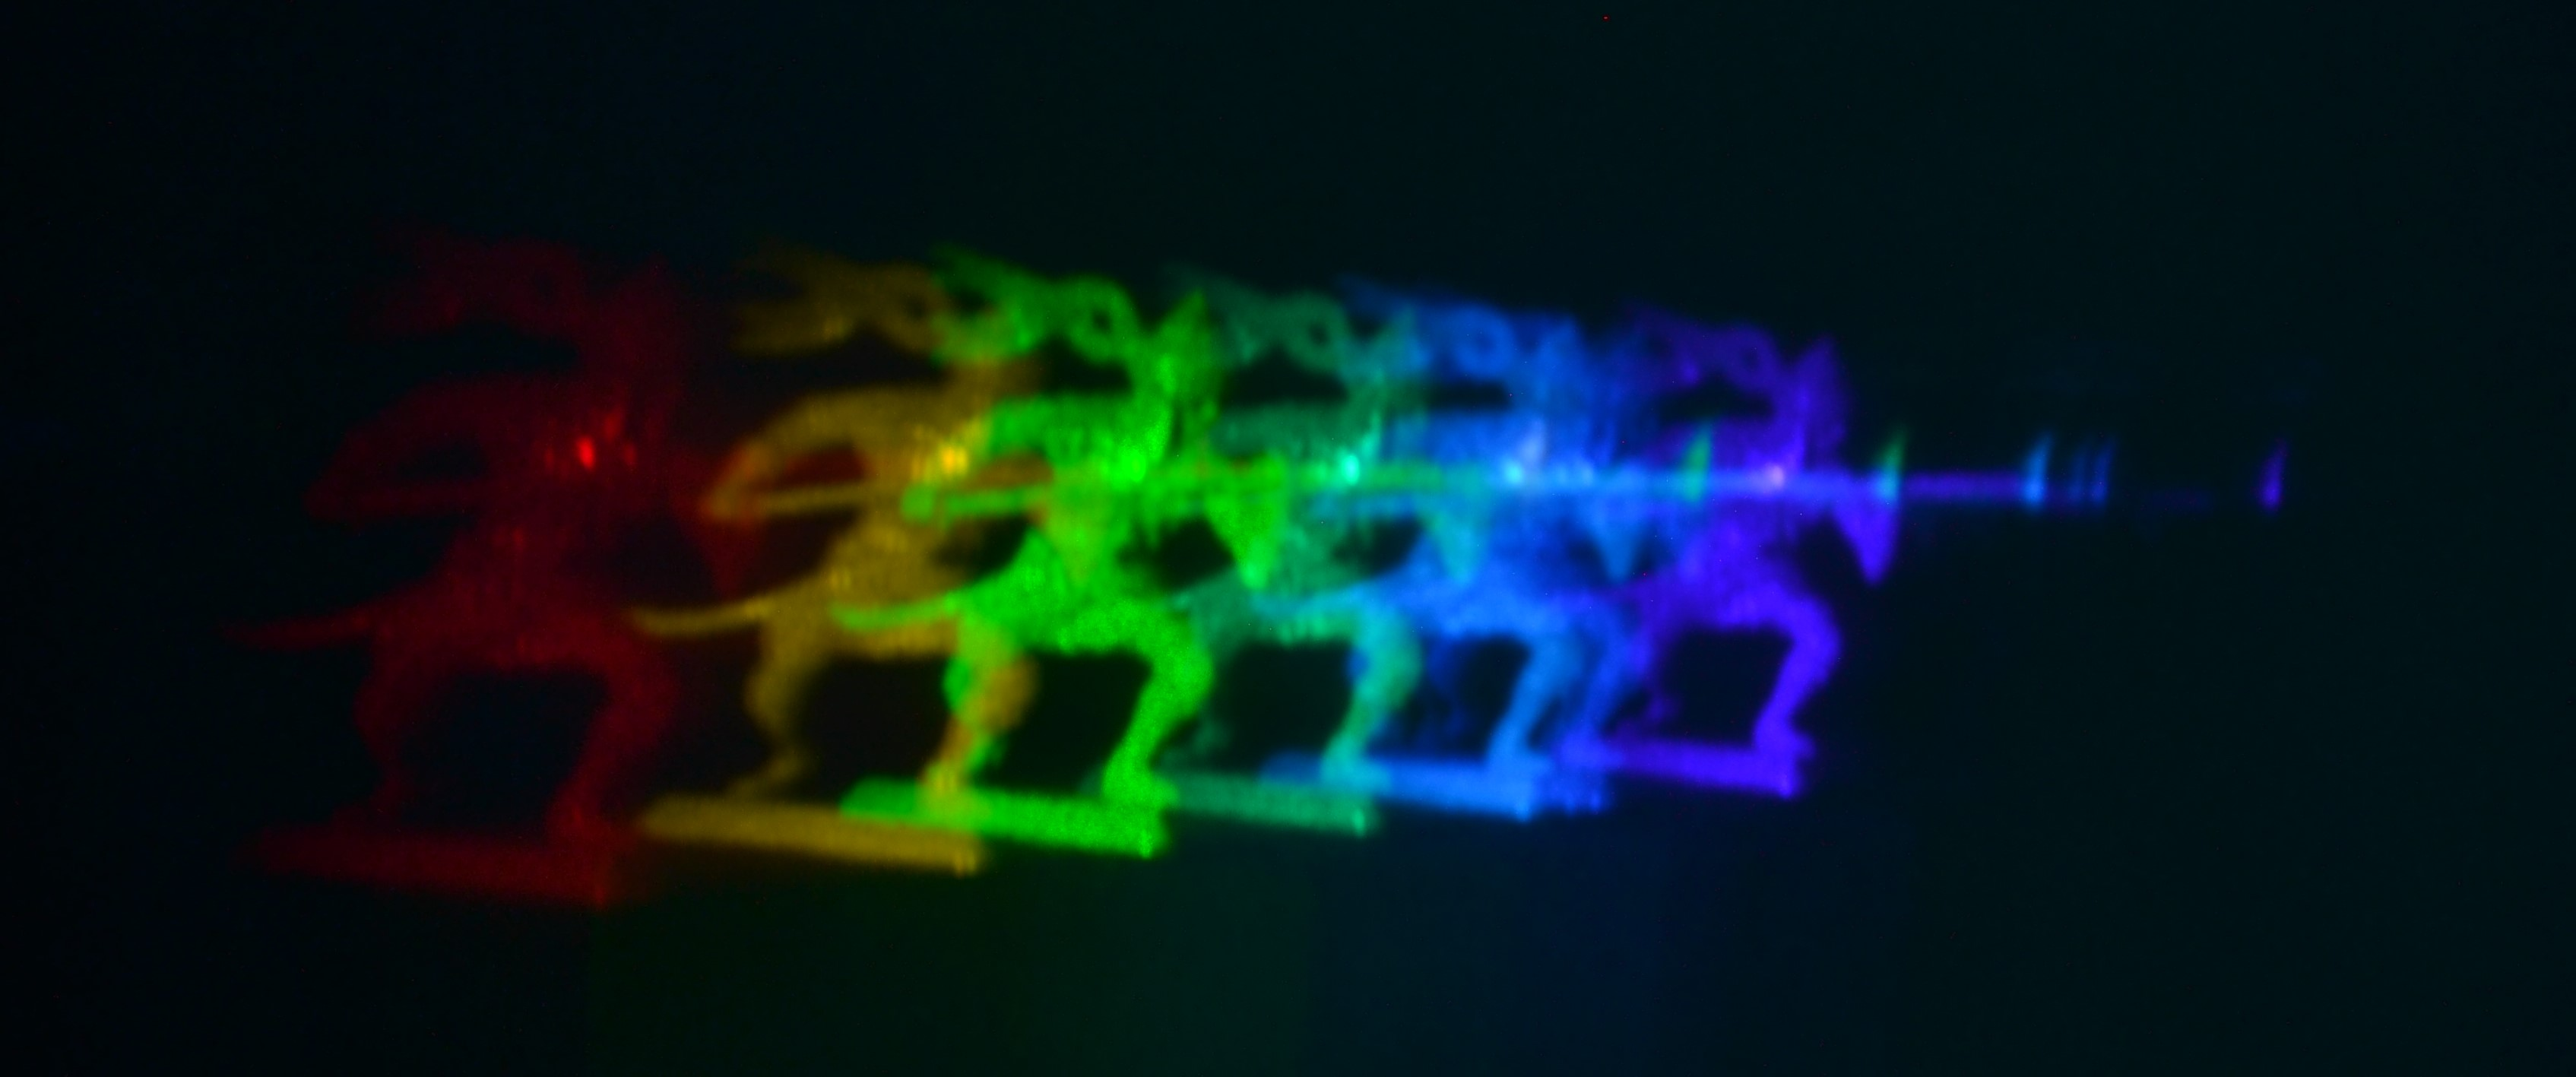
\includegraphics[width=\textwidth]{spettro}
\caption{}
\label{fig:spettro}
\end{figure}

	
\end{document}